\chapter{Measurement Journal: GPS Variance}
The intention of this journal is to measure the variance of the output of the ADIS16405 IMU.\todo{change to GPS}
\section{Equipment}
\begin{itemize}
\item ADIS16405\todo{change to GPS}
\item \todo{brand and specs of computer (AAU registration number if possible)}
\item APC220 Wireless communication Module
\end{itemize}

\section{Method}
A python script was implemented which logged the data which was accepted according to the protcol specifications chapter \ref{chap:Protocol}. The board on which the IMU is mounted is reading the data with a set delay between reads, and then bursting the data as soon as it has read. The data is timestamped when it is received by the python script. The script will keep running, receiving data, until it is cancelled. The system was then set to run overnight.\\
It was expected to see the GPS wander for some time, but then to reach some form of steadystate where the measurements would primarily be affected by the measurement noise. This was clearly observed, as seen on figure \ref{fig:measgps} \\
\begin{figure}
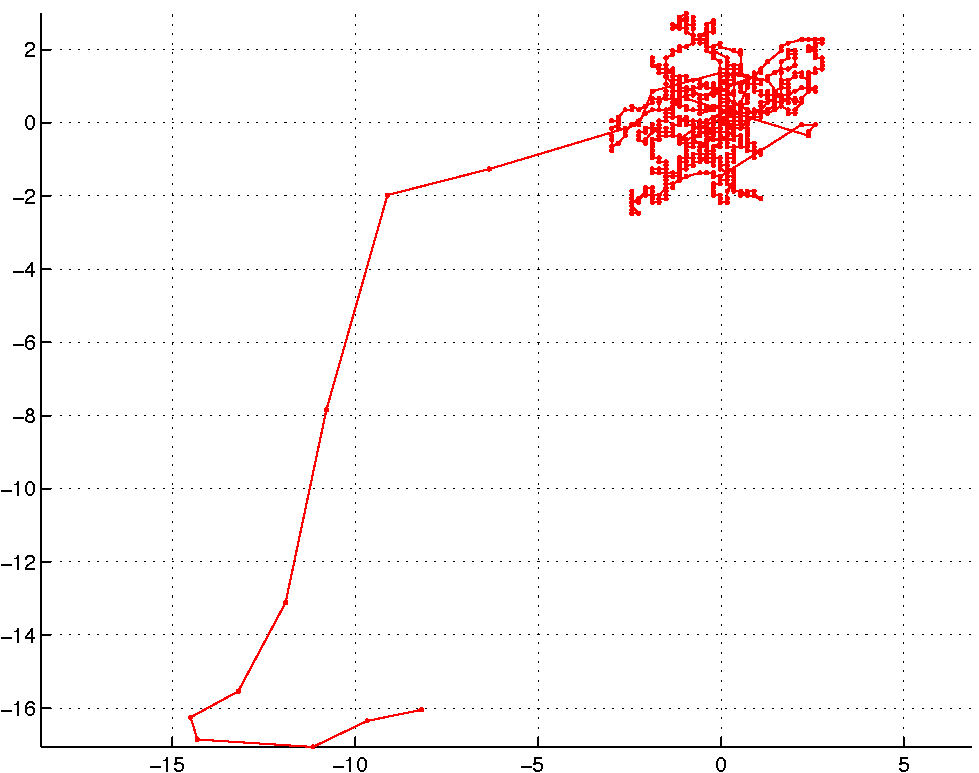
\includegraphics[width=\textwidth]{img/gpsmeas.pdf}
\caption{The GPS measurements, after being transformed into a local reference frame}
\end{figure}
\label{fig:measgps}

From an early trial run of the system it was discovered that the IMU would sporadically deliver measurements which were clearly wrong. Luckily all of the measurements were affected by this. Therefore it was possible to filter this by attaching the ADC of the IMU to ground, and then discarding the measurement when the ADC reads a high value.\\
The measurements are then input in Matlab, transformed into a local reference frame and the variances of the measurements are estimated, using the 'var()' function for the coordinate measurements. For the speed measurements, the unbiased sample variance formula as seen in equation (\ref{eq:measjournal:unbiassamplevariance}). Since the sample base is large, the effect of $\frac{1}{n}$ compared to $\frac{1}{n-1}$ is negligible, but the later should still be used, as the unbiased estimation is desired.

\begin{equation}
s^2_{N-1} = \frac{1}{N-1} \sum^N_{i=1}(x_i-\overline{x})^2
\end{equation}
\label{eq:measjournal:unbiassamplevariance}
\section{Measurements}
The measurements of the position can be found in gpsSDlog291112.log, while the speed data can be found in speedlog.log. As the speed measurements are not present in every sample from the GPS, the two files contain a different amount of samples. While position log contain 25220 measurements, the speedlog only contain 1690. This is however deemed sufficient for the variance estimate.
\section{Results}
The resulting variance of the GPS measurements were found to be 0.0026 $\frac{m}{s}$ for the speed measurements, while the variances for the position measurements were found to be 0.979 $m$ and 1.12 $m$, for the $x$ and $y$ position, respectively.